\documentclass{Article}
\usepackage[utf8]{inputenc}
\usepackage [danish]{babel}
\usepackage[a4paper, hmargin={2.8cm, 2.8cm}, vmargin={2.5cm, 2.5cm}]{geometry}
\usepackage{eso-pic} % \AddToShipoutPicture
\usepackage{graphicx} % \includegraphics
\linespread{1.2}
\usepackage{amsthm}
\usepackage{amsmath}
\usepackage{url}
\usepackage{tikz}
\usepackage{amsfonts}


\usepackage{listings}


\author{
\Large{dpj482}\\
    \\ \texttt{}
}

\title{
  \vspace{3cm}
  \Huge{CAC assignment 3} \\
  \Large{Christian Møllgaard}\\
}
\usepackage{natbib}
\usepackage{graphicx}

\begin{document}

%% Change `ku-farve` to `nat-farve` to use SCIENCE's old colors or
%% `natbio-farve` to use SCIENCE's new colors and logo.
\AddToShipoutPicture*{\put(0,0){\includegraphics*[viewport=0 0 700 600]{natbio-farve}}}
\AddToShipoutPicture*{\put(0,602){\includegraphics*[viewport=0 600 700 1600]{natbio-farve}}}

%% Change `ku-en` to `nat-en` to use the `Faculty of Science` header
\AddToShipoutPicture*{\put(0,0){\includegraphics*{nat-en}}}

\clearpage\maketitle
\thispagestyle{empty}

\newpage



%\lstinputlisting[language=Python, firstline=56, lastline=82]{nbodyphysics.py}

\section{Introduction}
The task of this assignment is to share the computation of CT-Reconstruction across several nodes mainly using pset. To reduce the amount of data sent between nodes, I decided to use multiprocessing with pypsets. 
\section{What have changed}
Here i will explain the changes to the original code. but split the explanations up in server, client and both categories.
\subsection{Both}
I have made a function, that set up all pset objects. This returns all the objects needed to communicate between nodes in the grid.

I create three psets. The first is for the shared data. The second is the job descriptions. The third is the result array.

To handle no more jobs, and I have introduced a "poison pill" job, that tells a node to shut down, because computation is done.
\subsection{Server}
I handle all time measurement on the server side, but only create the pset objects once, even though i measure times once for each voxel size. To accommodate this i calculate the time it takes to setup the psets and add those to all time calculations.

Firstly i move all the required data for this calculation using the psets. I only move it into the pset once. I then split all the work so every worker have almost the same workload, before adding the ranges for each worker to process as jobs. While doing this i spawn the workers. Then the poison pills are added to the job pset. When all this is done, the server wait for each worker to be done, and send a result back. The server then sums them up and axe the data and result pset, so they do not fill up the memory.

\subsection{client}
The client starts by getting all the data and saving them in global variables. A global result array is created. The client then creates a multiprocessing pool, with the desired amount of cpus. Then the client split the work by projection and send the jobs to the pool. There is no shared memory, because i could not make the shmarray work on the nodes.

When all sub processes are done, I sum the results and send them to the result pset. The client then checks for more jobs, but because will find a poison pill and stop. I created the poison pill, because so it can handle different kinds of splits, but a static split worked best for me.

\newpage
\section{Result}
I've run several different setups trying to mix the amount of nodes, and the amount of cpus run in parallel on each node. The results are shown in table 1. Not using the full capacity of the machine, and not spending to much time sending data between the machines seems to be the best thing. My speed up graph tops at 16 cpus and 4 nodes with a total of 64 cpus.
\begin{table}[]
\centering
\caption{Test results}
\label{my-label}
\begin{tabular}{|l|l|l|l|l|l|l|l|l|}
\hline
64 voxels & 128 voxels & 256 voxels & poolsize & nodes & total cpus & 64 speedup & 128 speedup & 256 speedup \\ \hline
9.8       & 69.04      & 536.19     & 1        & 1     & 1          & 1          & 1           & 1           \\ \hline
9.57      & 41.35      & 321.31     & 2        & 1     & 2          & 1.02       & 1.67        & 1.67        \\ \hline
13.15     & 42.07      & 322.98     & 1        & 2     & 2          & 0.75       & 1.64        & 1.66        \\ \hline
10.22     & 22.91      & 167.6      & 2        & 2     & 4          & 0.96       & 3.01        & 3.2         \\ \hline
5.82      & 13.35      & 90.02      & 4        & 2     & 8          & 1.68       & 5.17        & 5.96        \\ \hline
5.18      & 9.36       & 61.72      & 8        & 2     & 16         & 1.89       & 7.38        & 8.69        \\ \hline
7.87      & 7.01       & 39.04      & 16       & 2     & 32         & 1.25       & 9.85        & 13.73       \\ \hline
9.97      & 14.98      & 94.23      & 2        & 4     & 8          & 0.98       & 4.61        & 5.69        \\ \hline
6.19      & 10.35      & 58.39      & 4        & 4     & 16         & 1.58       & 6.67        & 9.18        \\ \hline
8.8       & 8.47       & 43.64      & 8        & 4     & 32         & 1.11       & 8.15        & 12.29       \\ \hline
5.56      & 7.5        & 34.57      & 16       & 4     & 64         & 1.76       & 9.21        & 15.51       \\ \hline
5.93      & 8.77       & 44.49      & 32       & 4     & 128        & 1.65       & 7.87        & 12.05       \\ \hline
11.15     & 10.73      & 48.13      & 4        & 8     & 32         & 0.88       & 6.43        & 11.14       \\ \hline
7.82      & 9.76       & 42.02      & 8        & 8     & 64         & 1.25       & 7.07        & 12.76       \\ \hline
7.84      & 10         & 45.02      & 16       & 8     & 128        & 1.25       & 6.9         & 11.91       \\ \hline
10.86     & 11.46      & 53.52      & 32       & 8     & 256        & 0.9        & 6.02        & 10.02       \\ \hline
9.13      & 18.32      & 105.72     & 1        & 8     & 8          & 1.07       & 3.77        & 5.07        \\ \hline
44.53     & 62.95      & 240.72     & 1        & 64    & 64         & 0.22       & 1.1         & 2.23        \\ \hline
\end{tabular}
\end{table}

Looking at the best results in the graph, it can be observed how the 64 voxels, were to small to benefit much from being sent to different nodes and could be optimised more locally. There is a clear limit to the amount of speedup gotten from increasing the amount of cpus for this job, using my code. 
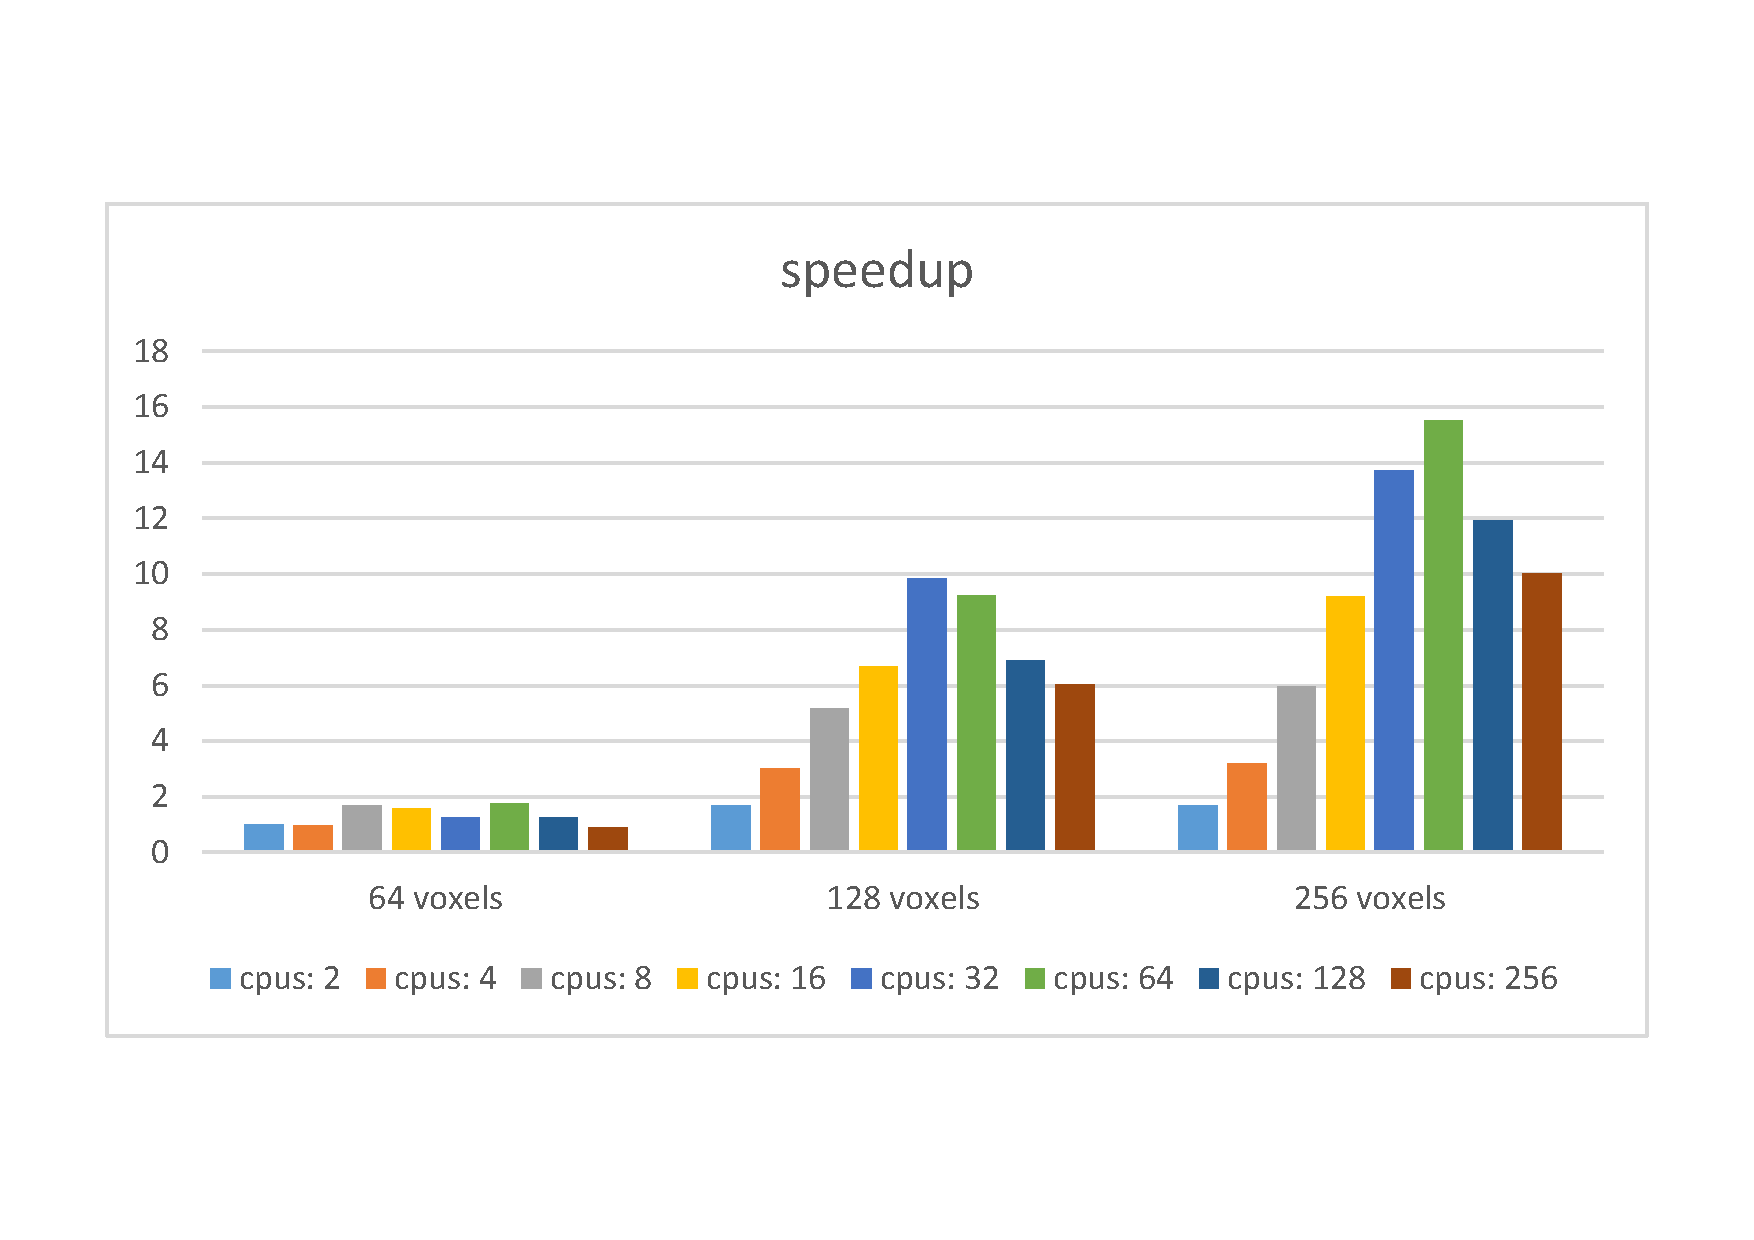
\includegraphics[clip, trim=0 3cm 0 3cm, width=1\textwidth]{speedup}\\

\subsection{What to improve}
I do not use shared memory for the multiprocessing part because of some namespace problems. If this could be solved, there would be saved some time in every process when it creates their own result arrays. It would mostly benefit when using larger amounts of cpus on each node, and could maybe fix the steep fail that happens after 32/64 cpus in the graph.
\section{conclusion}
It is easy to split problems up onto different nodes using pastsets, but it has some limitations when used for multiprocessing. It simply uses to much time on a lot of time setting everything up, so there is need for some extra multiprocessing to really benefit.
\end{document}
